% -*- Mode:TeX -*-

%% IMPORTANT: The official thesis specifications are available at:
%%            http://libraries.mit.edu/archives/thesis-specs/
%%
%%            Please verify your thesis' formatting and copyright
%%            assignment before submission. If you notice any
%%            discrepancies between these templates and the 
%%            MIT Libraries' specs, please let us know
%%            by e-mailing thesis@mit.edu

%% The documentclass options along with the pagestyle can be used to generate
%% a technical report, a draft copy, or a regular thesis. You may need to
%% re-specify the pagestyle after you \include cover.tex. For more
%% information, see the first few lines of mitthesis.cls. 

%\documentclass[12pt,vi,twoside]{mitthesis}
%%
%%  If you want your thesis copyright to you instead of MIT, use the
%%  ``vi'' option, as above.
%%
%\documentclass[12pt,twoside,leftblank]{mitthesis}
%%
%% If you want blank pages before new chapters to be labelled ``This
%% Page Intentionally Left Blank'', use the ``leftblank'' option, as
%% above. 

\documentclass[12pt,twoside]{mitthesis}
\usepackage{lgrind}
%% These have been added at the request of the MIT Libraries, because
%% some PDF conversions mess up the ligatures.  -LB, 1/22/2014
\usepackage{cmap}
\usepackage{graphicx}
\usepackage{braket}
\usepackage{lmodern}

\usepackage[T1]{fontenc}
\pagestyle{plain}

%% This bit allows you to either specify only the files which you wish to
%% process, or `all' to process all files which you \include.
%% Krishna Sethuraman (1990).

%\typein [\files]{Enter file names to process, (chap1,chap2 ...), or `all' to process all files:}
\def\all{all}
\ifx\files\all \typeout{Including all files.} \else %\typeout{Including only \files.} \includeonly{\files} \fi

\begin{document}

% -*-latex-*-
% 
% For questions, comments, concerns or complaints:
% thesis@mit.edu
% 
%
% $Log: cover.tex,v $
% Revision 1.9  2019/08/06 14:18:15  cmalin
% Replaced sample content with non-specific text.
%
% Revision 1.8  2008/05/13 15:02:15  jdreed
% Degree month is June, not May.  Added note about prevdegrees.
% Arthur Smith's title updated
%
% Revision 1.7  2001/02/08 18:53:16  boojum
% changed some \newpages to \cleardoublepages
%
% Revision 1.6  1999/10/21 14:49:31  boojum
% changed comment referring to documentstyle
%
% Revision 1.5  1999/10/21 14:39:04  boojum
% *** empty log message ***
%
% Revision 1.4  1997/04/18  17:54:10  othomas
% added page numbers on abstract and cover, and made 1 abstract
% page the default rather than 2.  (anne hunter tells me this
% is the new institute standard.)
%
% Revision 1.4  1997/04/18  17:54:10  othomas
% added page numbers on abstract and cover, and made 1 abstract
% page the default rather than 2.  (anne hunter tells me this
% is the new institute standard.)
%
% Revision 1.3  93/05/17  17:06:29  starflt
% Added acknowledgements section (suggested by tompalka)
% 
% Revision 1.2  92/04/22  13:13:13  epeisach
% Fixes for 1991 course 6 requirements
% Phrase "and to grant others the right to do so" has been added to 
% permission clause
% Second copy of abstract is not counted as separate pages so numbering works
% out
% 
% Revision 1.1  92/04/22  13:08:20  epeisach

% NOTE:
% These templates make an effort to conform to the MIT Thesis specifications,
% however the specifications can change. We recommend that you verify the
% layout of your title page with your thesis advisor and/or the MIT 
% Libraries before printing your final copy.
\title{Measurement of the Chiral-Odd Generalized Parton Distribution Functions through Non-Parametric Analysis of the Deeply Virtual Neutral Pion Electroproduction Cross Section at the Thomas Jefferson National Accelerator Facility at 10.6 GeV}

\author{Robert Johnston}
% If you wish to list your previous degrees on the cover page, use the 
% previous degrees command:
%       \prevdegrees{A.A., Harvard University (1985)}
% You can use the \\ command to list multiple previous degrees
%       \prevdegrees{B.S., University of California (1978) \\
%                    S.M., Massachusetts Institute of Technology (1981)}
\department{Department of Physics}

% If the thesis is for two degrees simultaneously, list them both
% separated by \and like this:
% \degree{Doctor of Philosophy \and Master of Science}
\degree{Interdisciplinary PhD in Physics and Statistics}

% As of the 2007-08 academic year, valid degree months are September, 
% February, or June.  The default is June.
\degreemonth{June}
\degreeyear{2023}
\thesisdate{May 18, 2023}

%% By default, the thesis will be copyrighted to MIT.  If you need to copyright
%% the thesis to yourself, just specify the `vi' documentclass option.  If for
%% some reason you want to exactly specify the copyright notice text, you can
%% use the \copyrightnoticetext command.  
%\copyrightnoticetext{\copyright IBM, 1990.  Do not open till Xmas.}

% If there is more than one supervisor, use the \supervisor command
% once for each.
\supervisor{Richard Milner}{Professor}

% This is the department committee chairman, not the thesis committee
% chairman.  You should replace this with your Department's Committee
% Chairman.
\chairman{Arthur C. Chairman}{Chairman, Department Committee on Graduate Theses}

% Make the titlepage based on the above information.  If you need
% something special and can't use the standard form, you can specify
% the exact text of the titlepage yourself.  Put it in a titlepage
% environment and leave blank lines where you want vertical space.
% The spaces will be adjusted to fill the entire page.  The dotted
% lines for the signatures are made with the \signature command.
\maketitle

% The abstractpage environment sets up everything on the page except
% the text itself.  The title and other header material are put at the
% top of the page, and the supervisors are listed at the bottom.  A
% new page is begun both before and after.  Of course, an abstract may
% be more than one page itself.  If you need more control over the
% format of the page, you can use the abstract environment, which puts
% the word "Abstract" at the beginning and single spaces its text.

%% You can either \input (*not* \include) your abstract file, or you can put
%% the text of the abstract directly between the \begin{abstractpage} and
%% \end{abstractpage} commands.

% First copy: start a new page, and save the page number.
\cleardoublepage
% Uncomment the next line if you do NOT want a page number on your
% abstract and acknowledgments pages.
% \pagestyle{empty}
\setcounter{savepage}{\thepage}
\begin{abstractpage}
% $Log: abstract.tex,v $
% Revision 1.1  93/05/14  14:56:25  starflt
% Initial revision
% 
% Revision 1.1  90/05/04  10:41:01  lwvanels
% Initial revision
% 
%
%% The text of your abstract and nothing else (other than comments) goes here.
%% It will be single-spaced and the rest of the text that is supposed to go on
%% the abstract page will be generated by the abstractpage environment.  This
%% file should be \input (not \include 'd) from cover.tex.



%{\Huge $\braket{\Psi | \Phi}$}
{\fontsize{180}{240} \selectfont  $\braket{\Psi | \Phi}$}

Deeply virtual exclusive reactions provide unique channels to study both transverse and longitudinal properties of the nucleon simultaneously, allowing for a 3D image of nucleon substructure. This presentation will discuss work towards extracting an absolute cross section for one such exclusive process, deeply virtual neutral pion production, using 10.6 GeV electron scattering data off a proton target from the CLAS12 experiment in Jefferson Lab Hall B . This measurement is important as exclusive meson production has unique access to the chiral odd GPDs, and is also a background for other exclusive processes such as DVCS, making the determination of this cross section crucial for other exclusive analyses.

\end{abstractpage}

% Additional copy: start a new page, and reset the page number.  This way,
% the second copy of the abstract is not counted as separate pages.
% Uncomment the next 6 lines if you need two copies of the abstract
% page.
% \setcounter{page}{\thesavepage}
% \begin{abstractpage}
% % $Log: abstract.tex,v $
% Revision 1.1  93/05/14  14:56:25  starflt
% Initial revision
% 
% Revision 1.1  90/05/04  10:41:01  lwvanels
% Initial revision
% 
%
%% The text of your abstract and nothing else (other than comments) goes here.
%% It will be single-spaced and the rest of the text that is supposed to go on
%% the abstract page will be generated by the abstractpage environment.  This
%% file should be \input (not \include 'd) from cover.tex.



%{\Huge $\braket{\Psi | \Phi}$}
{\fontsize{180}{240} \selectfont  $\braket{\Psi | \Phi}$}

Deeply virtual exclusive reactions provide unique channels to study both transverse and longitudinal properties of the nucleon simultaneously, allowing for a 3D image of nucleon substructure. This presentation will discuss work towards extracting an absolute cross section for one such exclusive process, deeply virtual neutral pion production, using 10.6 GeV electron scattering data off a proton target from the CLAS12 experiment in Jefferson Lab Hall B . This measurement is important as exclusive meson production has unique access to the chiral odd GPDs, and is also a background for other exclusive processes such as DVCS, making the determination of this cross section crucial for other exclusive analyses.

% \end{abstractpage}

\cleardoublepage

\section*{Acknowledgments}

I'd like to take this chance to acknowledge \newline
\newline

\vspace{2cm}

\begin{flushright}
    absolutely nobody
\end{flushright}

\begin{figure}[hbt]
	\centering
	 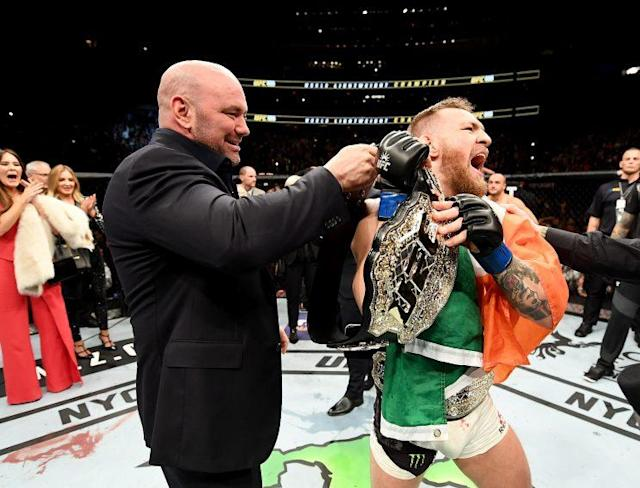
\includegraphics[trim={5cm 0 0 0.8cm} ,clip,width=.725995\textwidth]{templates/me.jpg}

\end{figure}

Lupe Fiasco, for inspiration, Nick Cambi for perspiration, and Inky Johnson for motivation.

joe jack Cathy Karen Dow (mit general services)
Ernie Kelsey
Tami
Messina
Rice
Miskimen
Joe (service guy from UMass)
All JLab hockey guys
Elton Smith JLab
the tech guy from JLab that was fat and crazy
Thesis Peter Charles axel Fabian jlab people
Fridericke Jentoft
Jan, ross, frank taylor for thesis




TO DO
-	Get a slide for Richard (best plot)
-	Need to include error bars (and bigger data points) on plot vs. T graph
-	compare chi square of clas12 and clas 6 data points
-	 
-	
Compare to other hall results (A, C)
Need to figure out discrepancy between my epsilon calculation and that of Pi0GKVegas.cpp
DONE
People to email:
Maurizio
Maxieme Dufrene
Kemal Tenzign

Remove low acceptance bins and rerun

Email Simonetta on easy as Pi!

igure out rosenbluth separation a la igor for statistical analysiss
need to reine code for grabbing nearest GK model fit because doing averaging doesn't seem to be a good idea




Official Repo: https://github.com/robertej19/clas12DVPiP
Local working dir: /mnt/c/Users/rober/Dropbox/Bobby/Linux/work/CLAS12/mit-clas12-analysis/theana/paragon/analysis/threnody
Local data dir: /mnt/d/GLOBUS/CLAS12
Simulation submission portal: %https://gemc.jlab.org/web_interface/index.php

For Fall DNP:

More notes for Thesis:
GK model link: 

 






%%%%%%%%%%%%%%%%%%%%%%%%%%%%%%%%%%%%%%%%%%%%%%%%%%%%%%%%%%%%%%%%%%%%%%
% -*-latex-*-

% Some departments (e.g. 5) require an additional signature page.  See
% signature.tex for more information and uncomment the following line if
% applicable.
% % -*- Mode:TeX -*-
%
% Some departments (e.g. Chemistry) require an additional cover page
% with signatures of the thesis committee.  Please check with your
% thesis advisor or other appropriate person to determine if such a 
% page is required for your thesis.  
%
% If you choose not to use the "titlepage" environment, a \newpage
% commands, and several \vspace{\fill} commands may be necessary to
% achieve the required spacing.  The \signature command is defined in
% the "mitthesis" class
%
% The following sample appears courtesy of Ben Kaduk <kaduk@mit.edu> and
% was used in his June 2012 doctoral thesis in Chemistry. 

\begin{titlepage}
\begin{large}
This doctoral thesis has been examined by a Committee of the Department
of Chemistry as follows:

\signature{Professor Jianshu Cao}{Chairman, Thesis Committee \\
   Professor of Chemistry}

\signature{Professor Troy Van Voorhis}{Thesis Supervisor \\
   Associate Professor of Chemistry}

\signature{Professor Robert W. Field}{Member, Thesis Committee \\
   Haslam and Dewey Professor of Chemistry}
\end{large}
\end{titlepage}


\pagestyle{plain}
  % -*- Mode:TeX -*-
%% This file simply contains the commands that actually generate the table of
%% contents and lists of figures and tables.  You can omit any or all of
%% these files by simply taking out the appropriate command.  For more
%% information on these files, see appendix C.3.3 of the LaTeX manual. 
\tableofcontents
\newpage
\listoffigures
\newpage
\listoftables


\chapter{On the Trento angle convention}

\iffalse
phi1 = angle(v3l,v3h)
phi2 = angle(v3l,v3g)
where if dot(v31,pro > 0,), phi1 =  360 - phi1
if  dot(v31,pro < 0,), phi1 =  phi1 I think check this

v3l = cross(beam,ele) = pe x pe'
v3h = cross(pro,vgs) = pp' x pgamma*
v3g = cross(vgs,pi0) = pgamma* x ppi0
ppi0 = pgamma1+pgamma2

vgs = (-Epx,-Epy, pbeam-df(EPZ) = (-pe'x, -pe'y, pbeam-pe'z) where pbeam = sqrt(beam-me^2)

angle = arccos(costheta(vec1,vec2))
costheta = v1*v2/sqrt(v1*v1*v2*v2)

Thus:
phi = arccos( (v3l dot v3h) / (mag v3l mag v3h) ) 
\fi
phi =    \footnotesize{$\cos^{-1} \left( \frac{ \left(p_{e} \times p_{e'} \right) \cdot \left( p_{p'} \times p_{\gamma^*} \right) }{ \lVert p_{e} \times p_{e'} \rVert \: \lVert p_{p'} \times p_{\gamma^*} \rVert} \right)$}

if dot(pe cross pe', pp') is greater than 0, then do 360 - phi = phi.
If we expand the above out, we get:
-pp'x*ez*ey' + py*ez*ex' is greater than zero
which we can reduce to 
-pp'x*ey' + py*ex' is greater than zero

By inspecting table below, we can see what this really amounts to, is the trento convention saying that we take the angle by measuring counterclockwise from the proton vector to the electron vector.


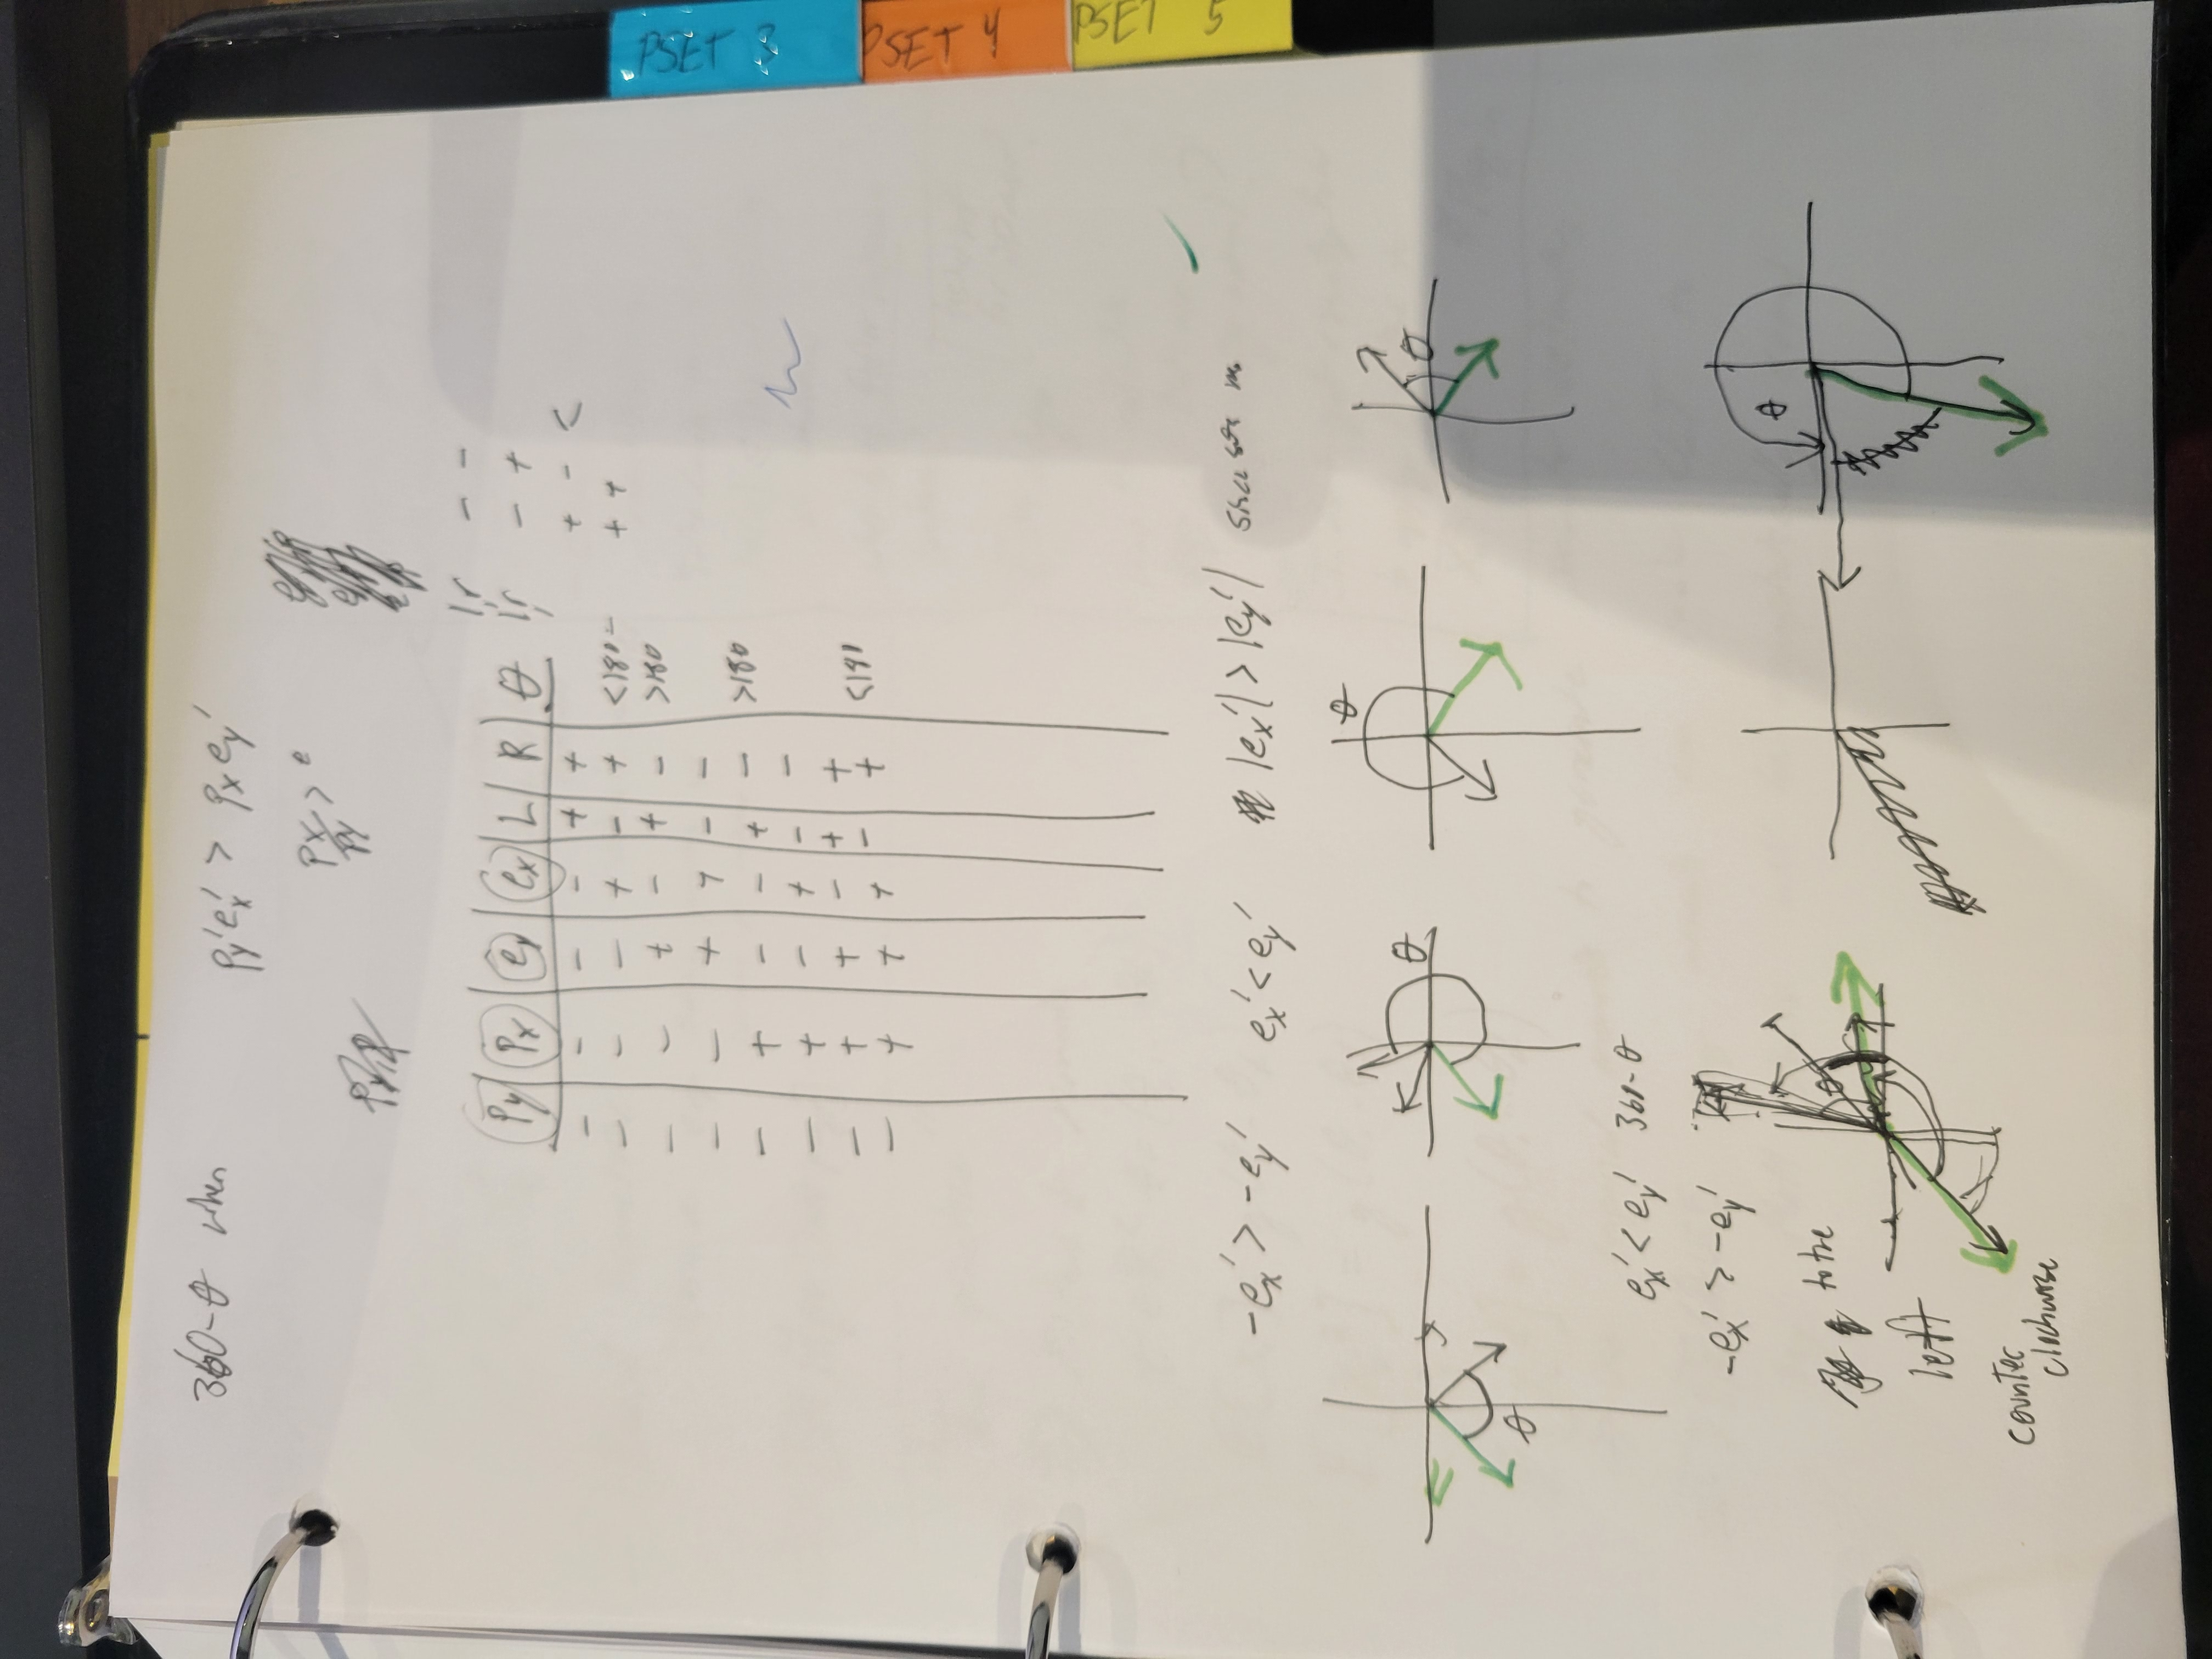
\includegraphics[width=0.9\textwidth]{basics/phi_math_1.jpg}
\section{Background}
Hi \cite{Bedlinskiy2014} see more in section ~\ref{ch1:bkrnd}

\include{chap2}
\appendix
\section{Full Cross Section Data}
To be completed

\section{Cross check between Andrey Kim and Bobby Johnston}

As an additional cross check, Bobby calculated a $DV\pi^0P$ beam spin asymmetry and compared to Andrey Kim's results. This check will not comment on any acceptance, luminosity, or virtual photon flux factor calculations, but does validate exclusive event selection criteria. By examining figure \ref{fig:bsa} we can see that agreement is reasonable, especially considering Bobby's calculation does not have sideband subtraction included.

\begin{figure}[hbt]
	\centering
	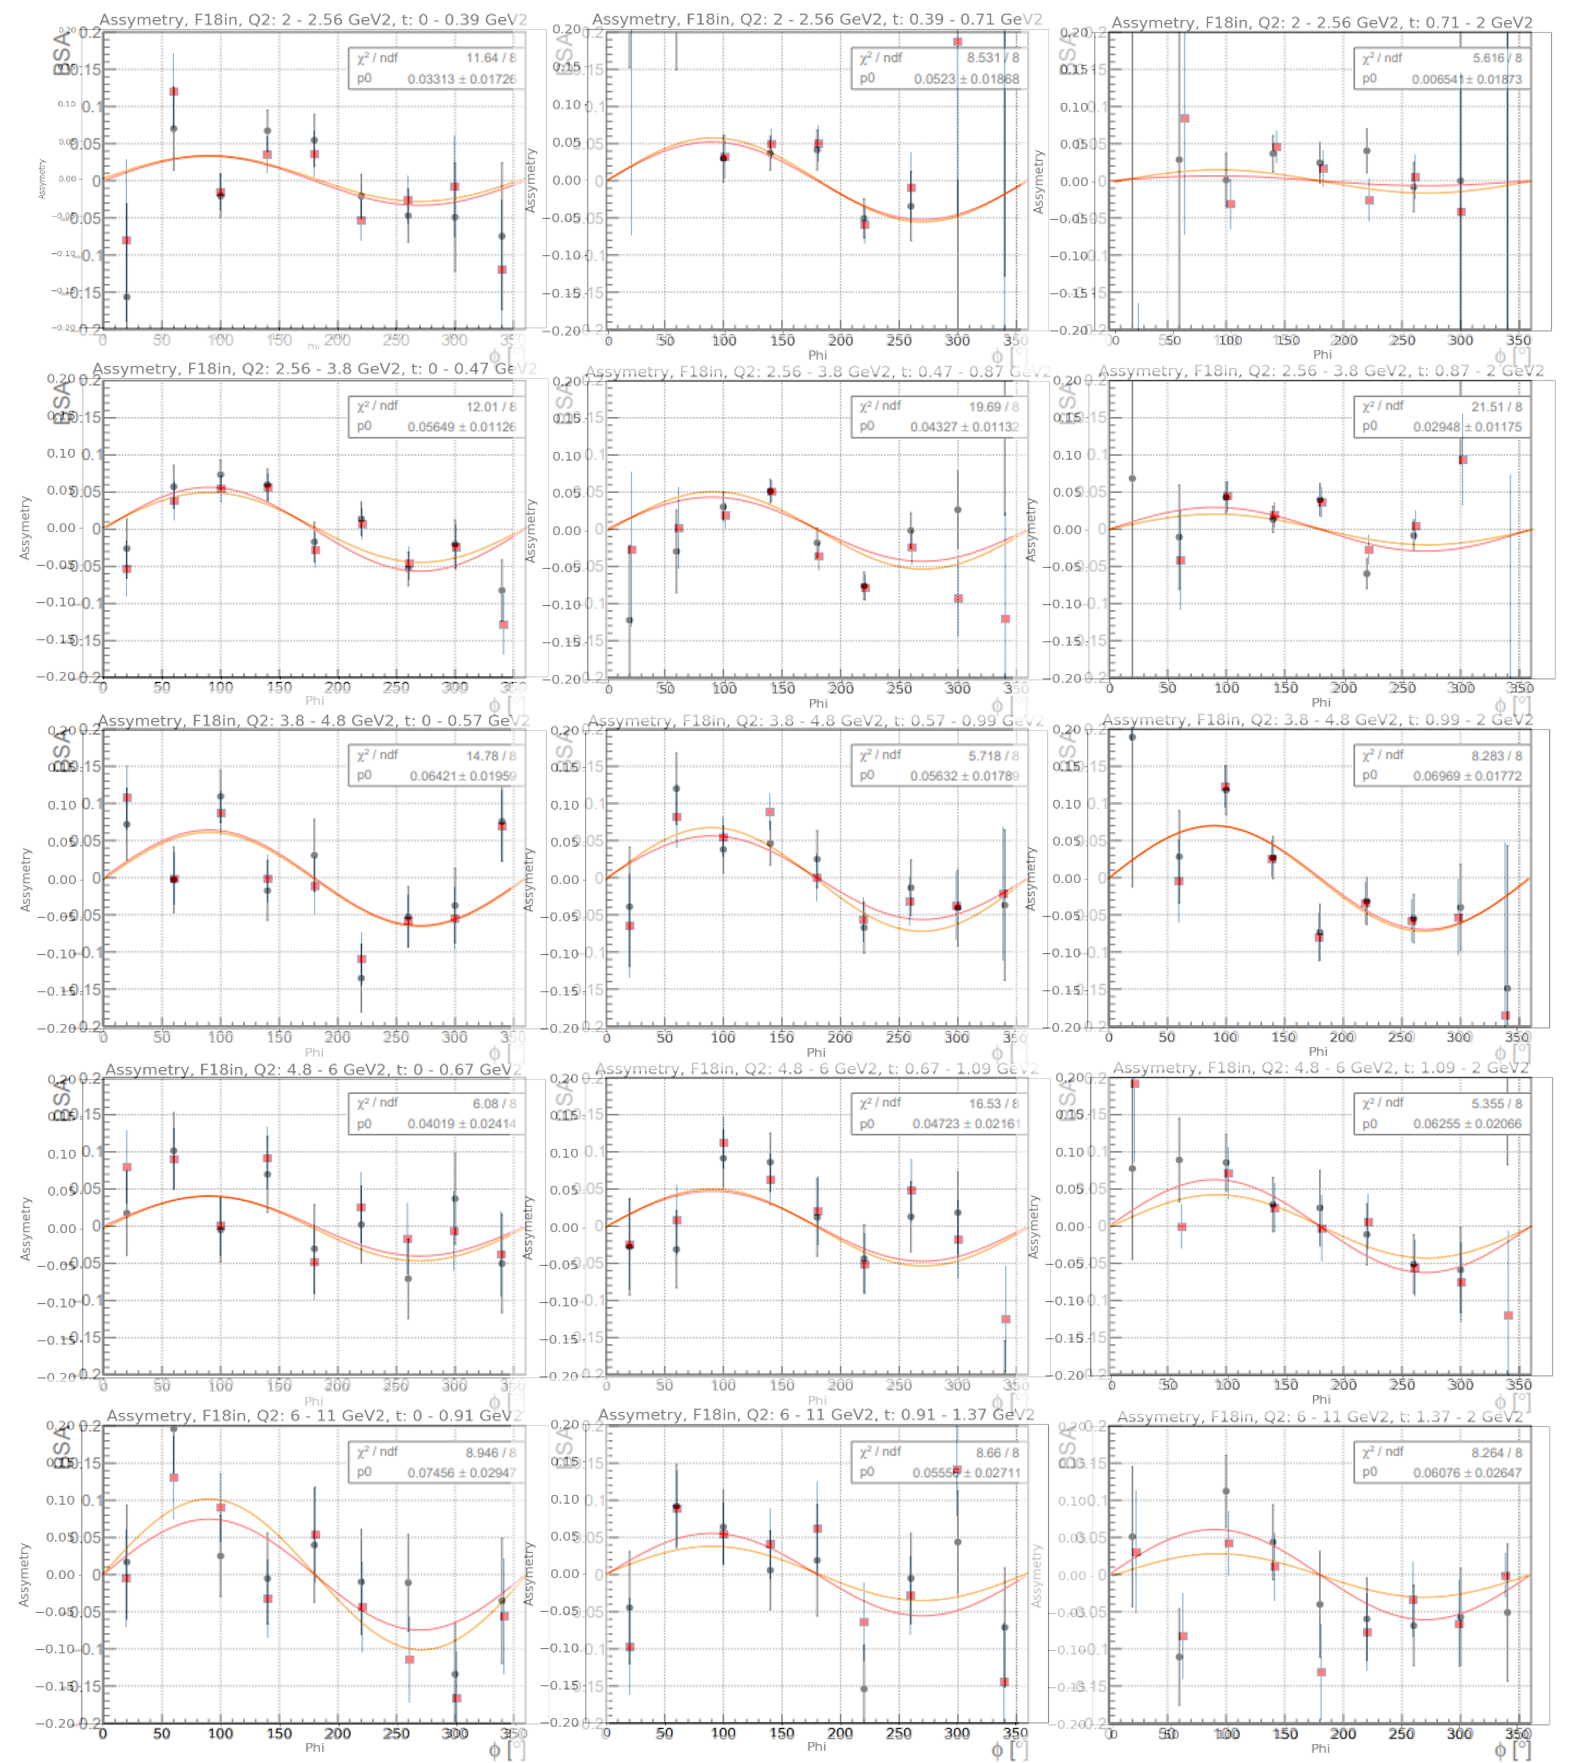
\includegraphics[width=0.75\linewidth]{Postamble/appb_pics/BSA.png}
	
	
	\caption{Overlay comparison of Andrey Kim's results (black datapoints, red fit line) and Bobby's results (red datapoints, orange fit line).}
	\label{fig:bsa}
\end{figure}


%% This defines the bibliography file (main.bib) and the bibliography style.
%% If you want to create a bibliography file by hand, change the contents of
%% this file to a `thebibliography' environment.  For more information 
%% see section 4.3 of the LaTeX manual.
\begin{singlespace}
\bibliography{bib/manrefs.bib}
\end{singlespace}

\end{document}

